\documentclass{article}
\usepackage[left=2cm, right=1cm]{geometry}
\usepackage{tikz}
\usetikzlibrary{backgrounds}

\begin{document}
\begin{figure} \begin{center}
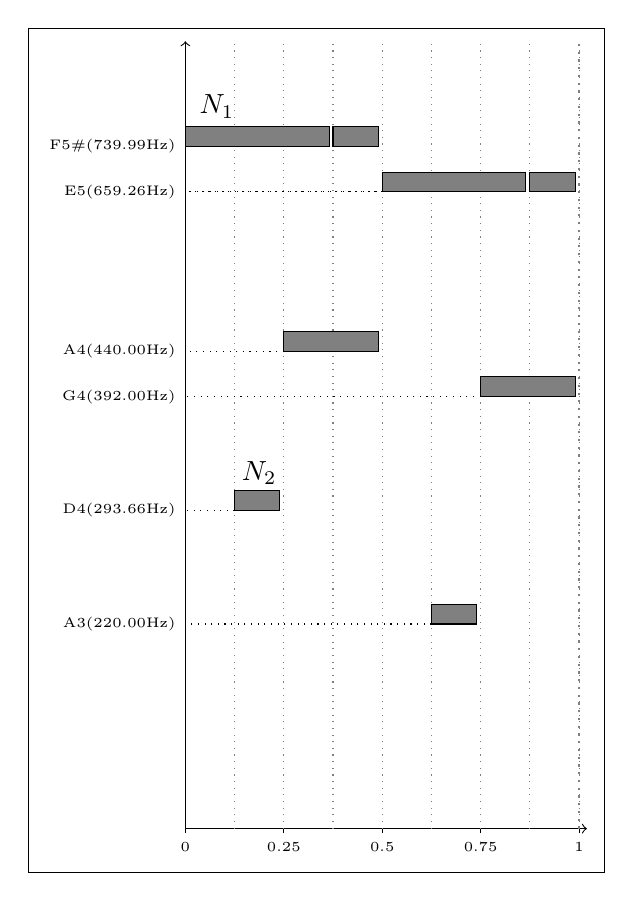
\begin{tikzpicture}[scale=5, show background rectangle]
    

    \draw[->] (0, 0) -- (1.02, 0);
    \foreach \x in { 0, 0.25, ..., 1.02 }
        \draw (\x, 0) -- (\x, -0.01) node[below]  {\tiny \x};
    \foreach \x in { 0.125, 0.25, ..., 1.02 }
        \draw[dotted, color=gray] (\x, 0) -- (\x, 2);
    \draw[->] (0, 0) -- (0, 2);
    
    \draw[fill=gray] (0.0, 1.7328679514) rectangle (0.365, 1.7828679514);
    \draw[dotted] (0.0, 1.7328679514) -- (0, 1.7328679514) node[left] {\tiny F5\#(739.99Hz) };
    \draw[fill=gray] (0.125, 0.808671710653) rectangle (0.24, 0.858671710653);
    \draw[dotted] (0.125, 0.808671710653) -- (0, 0.808671710653) node[left] {\tiny D4(293.66Hz) };
    \draw[fill=gray] (0.25, 1.21300756598) rectangle (0.49, 1.26300756598);
    \draw[dotted] (0.25, 1.21300756598) -- (0, 1.21300756598) node[left] {\tiny A4(440.00Hz) };
    \draw[fill=gray] (0.375, 1.7328679514) rectangle (0.49, 1.7828679514);
    \draw[dotted] (0.375, 1.7328679514) -- (0, 1.7328679514);
    \draw[fill=gray] (0.5, 1.61734342131) rectangle (0.865, 1.66734342131);
    \draw[dotted] (0.5, 1.61734342131) -- (0, 1.61734342131) node[left] {\tiny E5(659.26Hz) };
    \draw[fill=gray] (0.625, 0.51986038542) rectangle (0.74, 0.56986038542);
    \draw[dotted] (0.625, 0.51986038542) -- (0, 0.51986038542) node[left] {\tiny A3(220.00Hz) };
    \draw[fill=gray] (0.75, 1.09748303589) rectangle (0.99, 1.14748303589);
    \draw[dotted] (0.75, 1.09748303589) -- (0, 1.09748303589) node[left] {\tiny G4(392.00Hz) };
    \draw[fill=gray] (0.875, 1.61734342131) rectangle (0.99, 1.66734342131);
    \draw[dotted] (0.875, 1.61734342131) -- (0, 1.61734342131);
    \draw[dotted, thick, color=gray] (1, 0) -- (1, 2);

    \node[above] (note1) at (0.08, 1.78) { $N_1$ };
    \node[above] (note2) at (0.1875, 0.85) { $N_2$ };

\end{tikzpicture}
\end{center} \end{figure}
\end{document}
    
